\chapter{Literature review}
This chapter will present the literature study that has been carried out and presenting the different topics to the reader.


%This chapter includes sections about lane detection in general and what modalities are the most frequently used. Image processing including edge detection and hough transform. MCS. Information about the board  (EMC2 and zedboard).

\section{SAE level}
When talking about Advanced Driver Assistance Systems (ADAS) and autonomous vehicles it is important to define what it actually means. SAE International is a professional association and standards developing organization for transport industries. They have developed a new standard for autonomous driving called  "J3016: Taxonomy and Definitions for Terms Related to On-Road Motor Vehicle Automated Driving Systems,”. This standard defines six levels of driving automation, from no automation to full automation and is described more in detail in table \ref{SAE2} below \cite{SAE} \cite{SAEweb}. 


\begin{table}[H]
\centering
\caption{SAE levels description}
\label{SAE2}
\begin{tabular}{@{} lll}
\toprule
\textbf{Level} & \textbf{Name} & \textbf{Description}  \\
\midrule
\\[-1em]
 0 & No Automation & The human does all the work \\
 \\[-1em]
\rowcolor{black!15} 1 & Driver Assistance & \pbox{7cm}{The vehicle help out by doing a single task. One example is a cruise control where the car holds a reference speed} \\
\\[-1em]
 2 & Partial Automation & \pbox{7cm}{The first level that is considered as an automated driving system. In this level the vehicle is able to make decisions as overtaking other vehicles and navigating. In this level humans are only the fall-back option if something fails the vehicle will request the human to intervene } \\
 \\[-1em]
 \rowcolor{black!15} 3 & Conditional Automation & \pbox{7cm}{The first level that is considered as an automated driving system. In this level the vehicle is able to make decisions as overtaking other vehicles and navigating. In this level humans are only the fall-back option if something fails the vehicle will request the human to intervene} \\
 \\[-1em]
 4 & High Automation & \pbox{7cm}{In level 4, the vehicle is able to operate entirely by it self for the first time, there does not need to be any human behind the wheel as a fall-back. What differs this level from full automation is that it is on a geographically limited area like a center of a town, company area or college campus. } \\
 \\[-1em]
 \rowcolor{black!15} 5 & Full Automation & \pbox{7cm}{Level 5 is where full automated driving is reached. The vehicle can handle all operating modes. There is no steering wheel nor pedals. Just let the vehicle know where you want to go.} \\
\bottomrule
 \end{tabular}
\end{table}


When developing automated vehicles there are many functional safety requirements that must be fully verified and validated. One importance area is the vehicle actuation systems which are totally controlled by electronic systems. As the actuators are controlled by electronic systems they are strongly linked to other so called by-wire systems. Two examples are drive-by-wire and brake-by-wire. These systems do not have any mechanical coupling between the different elements but instead utilize sensors that read position of the brake pedal or steering wheel. In the development of these systems aspects as redundancy of the ECUs, sensors, actuators and power supply is required \cite{stolte2016safety}. 	The standard ISO 26262 is the most recent standard available concerning functional safety of electrical systems in the automotive industry. The standard requires determination of safety goals as part of hazard analysis and risk assessment. Once all the safety goals are defined, then functional safety requirements can be formulated.\\

According to Stolte \cite{stolte2016safety} it is needed to adopt measures that go beyond the state-of-the-art of modern production vehicles for ensuring functional safety of automated vehicles. The authors point out that despite the importance of series deployment of automated vehicles, there is not much discussion about safety requirements within the ITS community.  


\section{Lane keeping}
In its basic setting the lane detection problem seems like a simple one. The only thing needed is to detect a host lane and only for a short distance ahead.

For a human driving may seem like a simple process where two basic tasks are involved. The first is to keep the vehicle on the road and the second to avoid collisions. But in reality driving is not so trivial, a driver need to continuously analyze the road scene and choose and execute the appropriate maneuvers to deal with the current situation. To help the drivers do these tasks Driver Assistance Systems (DAS) have been developed. These systems can help the driver to perceive the blind area in the road for an example. An extension is the Advanced Driver Assistance System (ADAS) which can perform basic tasks like: Lane following, Lane keeping assistance, Lane departure warning, lateral control, intelligent cruise control, collision warning and ultimately autonomous driving.\\

The main bottleneck in the development of ADAS systems is the perception problem, which has two elements: road and lane perception, and obstacle detection. This degree project focuses on the first element and investigates the current state of the art research.\\

A simple Hough transform-based algorithm solves the problem in 90\% of highway cases \cite{BarHillel2014}. 
But the impression that the problem is easy is misleading and building a useful system requires a huge R\&{D} effort. One of the reasons is the high reliability demands. In order to be useful the system needs to reach very low error rates. The exact amount of acceptable false alarms of a lane departure warning is still a subject of research \cite{BarHillel2014}. At 15 frames per second, 1 false alarm per hour means only one error in 54,000 frames.\\

One factor that makes ADAS hard to implement on large scale is the large amount of different conditions that has to be taken care of. The main sources for condition diversity are:
\begin{itemize}  
\item lane and road appearance
\item image clarity issues
\item poor visibility conditions
\end{itemize}

When driving on freeways or large highways the road scene appearance diversity is minimized which makes it easier to implement lane detection functions and ultimately automated driving. This is one of the reasons why long haul trucks are the focus of a large portion of the research concering autonomous driving. 

\subsection{Modalities for environment perception}
In this section the modalities used for road and lane detection will be described more in detail.\\

Today there are several different sensing modalities used for lane detection. Some examples are monocular vision, stereo vision, LIDAR, IMU data, GPS.

\subsubsection{Monocular vision}
Vision is the most prominent research area due to the fact that road signs/markings are made for human vision. Vision sensors provides good position estimation on the road without the need for any other modalities. However, there are situations when vision sensors simply cannot perform well, for example in extreme weather conditions or when driving off-road. In this kind of situations it is possible to use sensor fusion with other sensor modalities to provide a better position estimate, and it is the reason why LIDAR and GPS are important compliments to vision for reaching full autonomous driving.\\

The monocular vision system is frequently used for road and lane detection. It is more simply put one camera mounted on the vehicle. The required resolution can be derived from $$N_p = \frac{Cd}{w}$$where $N_p$ is the number of horizontal pixels, $C$ is the camera field of view width in radians. $w$ is the lane mark width in meter \cite{BarHillel2014}.\\

When humans drive we continuously look at the road boundaries, the lane markings and the road texture among other things. These road boundaries are designed so that they should be visible for human drivers in all driving conditions. Self driving vehicles that are supposed to share the road with human drivers will therefore most likely have to rely on the same perceptual cues as humans.

\subsubsection{LIDAR}
Light detection and ranging (LIDAR) is a modality that has been used to a large extent in the development of autonomous vehicles for research purposes. The LIDAR measures the environment around the vehicle in 3D. The LIDAR sends out light pulse and measures the time for it to come back. As it is an active light source it is not dependent of having good natural lighting as with a regular camera.\\

LIDAR sensors can perform well in certain situations for example in rural areas to detect road boundaries, \cite{BarHillel2014} but are not well suited for multilane roads without vision data. As the LIDAR only measures 3D structures it is not able to detect road markings, although some research have been done on intensity measurement with LIDAR \cite{huang2009finding} \cite{kammel2008lidar} which would make it possible to detect line markings to some extent. One huge drawback with this modality is that the sensors are still very expensive and thus not yet an alternative for implementation in regular passenger vehicles.

\subsubsection{Stereo imaging}
Stereo imaging is the use of two cameras instead of one camera in order to obtain 3D information about the surrounding. It is a step in between monocular vision and LIDAR as it is much cheaper to implement than LIDAR but generally performs less good in terms of accuracy and reliability.  Also the stereo imaging system generally requires greater processing power and is more prone to errors compared to LIDAR. 


\subsubsection{GPS, IMU}
Geographical information system (GPS) is currently widely used for navigation systems. According to Wing \cite{wing2011} current commericial consumer grade GPS recievers can achieve an accuracy of 1.5-5 m. Which works sufficiently for map navigation when a human drives the vehicle but is simply not accurate enough to fully control a vehicle only based upon the GPS. Also the GPS does not give any information about the environment, e.g. other vehicles or pedestrians. This means that GPS will always need to be supplemented by a camera or LIDAR.\\
 
One problem with GPS is the reliability. GPS requires connection with enough satellites to function properly and that connection can be lost due to many reasons. Some level of lost connection can be tolerated by using inertial measurement unit (IMU). With the IMU it is possible to calculate current position and integrate with the GPS to get a more reliable estimation when the connection to satellites is weak.

\section{Flowchart of image processing}

\begin{figure}[H]
  \includegraphics[width=\textwidth]{./img/flow.png}
  \centering
  \caption{Flowchart of a general lane detection system}
  \label{fig:Software architecture of the EMC2 platform}
\end{figure}

\subsection{Image acquisition}
The image acquisition typically comes from a camera that is mounted in the center of the vehicle.

\subsection{Preprocess}
The preprocess is a step where the image is prepared for the next steps in terms of image resolution, where a lower image resolution is often preferred due to the high computational load that high resolution images bring \cite{Yenikaya:2013:KVR:2522968.2522970}. Everything that is not part of the region of interest (ROI) is often removed. This typically means removing the region above the horizon. Often gray-scale images are preferred over color images due to reduced data load \cite{Yenikaya:2013:KVR:2522968.2522970}. Removal of unwanted disturbances such as shadows are often done in the preprocess. As mentioned in the section about road models, inverse perspective mapping is commonly done in the image preprocess to get rid of the perspective effect \cite{bertozzi1998gold}.

\subsection{Feature extraction}
There are several features that can be used for road and lane detection. The most typically used are color, texture and edges. For structured roads with clear line markings the edges are the most common feature used for lane detection. An edge is defined as the gradient of the intensity function \cite{Yenikaya:2013:KVR:2522968.2522970}. The output of an edge based method are candidates for lane boundaries, since edge based methods are able to find where the image brightness changes sharply. There are some well known edge detection methods (Prewitt, Roberts, Sobel), but one method called Canny edge detector stands out and is still, 30 years after it was first developed, considered a state-of-the-art edge detector, some even mean that it is an optimal edge detector algorithm \cite{bhadauria2013comparison}. A general process of operations that occur in the canny edge detector starts with applying a gaussian filter to smooth the image in order to remove noise. The next step is to scan the image for intensity gradients with a gradient operator and then apply a filter to supress noise but keep edges in the image. Then the image is analyzed for non-maxima points to further remove pixels that are not actual edges in the image. Next step is to treshold the image and lastly finalize the detection of edges by a hysteresis treshold which supresses all the weak edges that are not connected to other edges.\\

Hough transform (HT) is then applied to the image in order to determine if there is an edge at one certain pixel or not. The Hough transform was originally invented 1962 and has since then been refined to the way it is universally used today. The HT works by converting the white pixels from the thresholded input image to points in the parameter coordinate space, meaning they will be represented using a direction theta and distance r instead of x an y.\\

Each point in the parameter space has a count, and each point in the image space has a vote. Edge pixels with the same theta and r value are assumed to define a line in the image. To compute the frequency of each line theta and r are put in a number of so called bins.  When all the edge pixels have been converted to parameter space these bins can be analyzed and the ones with the most amount of votes are the most prominent lines in the image. Usually a threshold is set where counts that does not exceed the threshold are ignored and only the most prominent lines are accepted \cite{davies}.

\subsection{Road model}
The majority of lane detection systems initially propose a model of a road. This model can be both something simple as straight lines or more complex splines. Some researchers make the assumption that the road is two parallel lines in the image, this can be done after an operation called inverse perspective mapping, which produces an bird's-eye view  perspective \cite{bertozzi1998gold}. One other common method is to assume that the lanes have a common vanishing point where the both lanes meet and use that as a reference for the lines in the image \cite{Yenikaya:2013:KVR:2522968.2522970}\cite{jingyu2013lane}. Both these two perspectives can be seen below in figure \ref{fig:Inverse perspective mapping and vanishing point perspective}

\begin{figure}[H]
  \begin{subfigure}[b]{0.50\textwidth}
    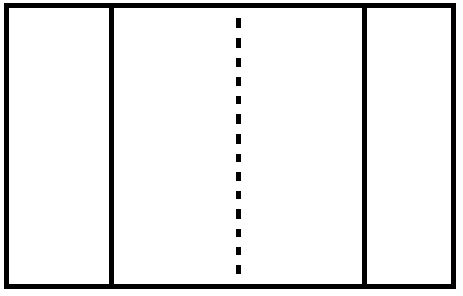
\includegraphics[width=\textwidth]{./img/IPM.png}
    \caption{\label{fig:Inverse perspective mapping}Inverse perspective mapping}
  \end{subfigure}
  \begin{subfigure}[b]{0.50\textwidth}
    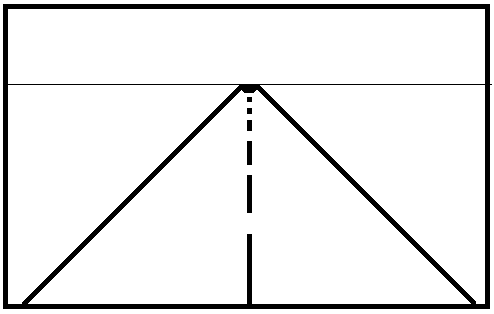
\includegraphics[width=\textwidth]{./img/Vanishingpoint.png}
    \caption{\label{fig:Vanishing point}Vanishing point}
  \end{subfigure}
  \caption{\label{fig:Inverse perspective mapping and vanishing point perspective}Road model in two different perspectives}
\end{figure}

\subsection{Model fitting}
As mentioned in the road model section, very often a road model is used and fitted to the observed information from the feature extraction section.\\

The extracted data from the previous step would typically contain both inliers, i.e. data that can be fitted to a line, and outliers, i.e. data that cannot be fitted onto the same line \cite{raguram2008comparative}. Assuming that the extracted data from previous steps contains data that can be fitted to one of the models chosen initially, several different approaches have been proposed for model fitting \cite{BarHillel2014}. Some researchers use least squares method, which is a mathematical procedure to fit a set of observed values to a function. The idea behind the method is to construct a function in such way so the sum of the difference between the observed value and the data points is minimized \cite{LS}.\\

Other research propose the use of "RANdom SAmple Consensus", known as the RANSAC algorithm \cite{huang2009finding}\cite{aly2008real} \cite{li2013lane}. This method is stated to be superior to least squares method due to its ability to fit a line to the inliers only, without any influence of the outliers on the result. The disadvantage with this method is that the computational time usually is longer compared to least squares method and is very dependent on the amount of outliers in the image \cite{RANSAC}.


\subsection{Time integration}
The last step that is important for a reliable lane detection system is to be able to incorporate some knowledge from previous frames. This is done in order to increase the reliability of the system and decrease the computational load.

\subsection{Lateral control}
Here I will write about lateral control

\section{Platooning}
As the traffic intensity increases in the world, the problem with traffic congestion comes with it. In and around large cities today there are already huge problems due to heavy traffic. The situation leads to increasing emissions of greenhouse gases such as carbon dioxide. One way to ease the problem of traffic congestion and reduce the fuel consumption of vehicles is vehicle platooning. The concept of vehicle platooning is to reduce the distance between the vehicles on the road and thus reducing the wind resistance acting on each vehicle. Today most of the research cover the topic of heavy duty vehicles (HDV), where trucks are used to form a platoon on highways. Modern commercially available driver assistance systems such as adaptive cruise control use radar measurements to know relative distance and velocity to preceding vehicle and adjusts its own velocity automatically. This strategy works sufficiently good if the distance between the vehicles is long enough due to delays from measurements of the preceding vehicle to actuation of accelerating or braking torque at the wheels.\\

One effort to reduce the distance between the vehicles in the platoon while maintaining the safety requirements is to send a brake signal through wireless communication to the other vehicles in the platoon. This would allow for a faster actuation of the brakes compared to only using radar. In research done by \cite{alam2014guaranteeing}, it is stated that if two identical vehicles are in a platoon on a highway road driving 90 km/h they can hold a minimum relative distance from each other of 1.2 m without endangering safety. In a scenario where a worst case delay of 500 ms is present in the system a minimum of 2 m distance should be kept. This distance is significantly shorter than what a modern adaptive cruise control achieves in order to keep a safe distance to preceding vehicle.\\


%\section{Convolutional Neural Networks}


\section{OpenCV}
OpenCV is an open source computer vision and machine learning software library. The library has a large amount of optimized algorithms for computer vision. A few areas where OpenCV is used are face recognition, object detection, tracking of moving objects and lane detection. Because OpenCV is a BSD-licensed product, it is free to both utilize and modify the code by companies all over the world. Companies like Google, Microsoft, Intel, Honda and Toyota employ the library for use in various different applications. OpenCV has C++, C, Python, Java and Matlab interfaces and supports all the major operating systems \cite{opencv}.\\

In this project several OpenCV funtions have been utilized mainly in the image processing part. More information about how it is implemented comes in next section.

\section{Mixed-criticality systems}
A trend in modern embedded systems is to take advantage of all the processing power available in a multicore processor chip. This can be done by combining different subsystems onto one chip which makes it possible to achieve higher CPU utilization and thus reduce hardware cost and power consumption. Sometimes these embedded systems contain components of different criticality. For the automotive industry that this thesis focuses on one example could be to run the ADAS and the infotainment system of the vehicle on the same electric control unit (ECU). If these two components are integrated onto a single hardware platform, the response time of the ADAS system should not be affected of the infotainment system. By scheduling these two components onto the same computing platform one creates a mixed-criticality system.\\

Each industry field (automotive, aerospace, railway, etc) has certain safety and security regulations that the mixed criticality systems needs to comply with. There are several different criticality levels in each industry that depend on elements such as environment of operation and danger to human life\cite{zaki2016}. According to Thane \cite{SIL}, safety can be defined as the absence of unacceptable risk. A system is safe if the risk associated with the system is acceptable. 


\subsection{Scheduling}
Every task that is implemented has a worst-case execution time (WCET). This is the maximum amount of time that the task can take to execute on the hardware platform. The WCET is used for guaranteeing that the temporal constraints will not be violated.\\

A scheduler can be either preemptive or non-preemptive. If the scheduler is preemptive, it can interrupt a task during execution if a task with higher priority is ready for execution, a non-preemptive scheduler will wait for the task to complete \cite{RTSS}. Some of the most common scheduling algorithms are:

\subsubsection{Fixed priority}
Every task has a fixed priority assigned by the developer and the processor will execute the highest priority task of those that are ready to be executed. 
\subsubsection{Earliest deadline first}
Earliest deadline first is a dynamic scheduling algorithm that always checks which task in the queue has the shortest time to its deadline and executes that task next.
\subsubsection{Rate-monotonic}
Rate-monotonic scheduling is an static priority scheduler where the priority of the tasks are assigned according to the task cycle time. The highest priority task will be the one with shortest cycle time and the lowest priority task will be the one with longest cycle time.
\subsubsection{Deadline-monotonic}
Deadline-monotonic priority is just like rate-monotonic a static priority scheduler with the difference that the priority is assigned according to deadline instead of cycle time. The task with the shortest deadline will be the one with highest priority.